\section{Design for Learning}

%\citep{effectivelearning-robert}
%\citep{learning-krathwohl}
%\citep{learning-ucla}

This first section deals with considerations on how to design for learning in regards to entrepreneurship education.

The following sections, are about how to design for effective learning, by designing for the mind, cognitive psychology.

Cognitive psychology deals with how our brain works in regards to our memory.

The section presents strategies and techniques to design learning for the mind, and what needs to be considered.

Two aspects are especially relevant when it comes to education: how humans learn (the first four sections), and how humans forget (the two last sections).

In how humans learn, the purpose is to find the most powerful strategies and techniques to design effective learning (mapping educational objectives, how to build skills, pattern-matching techniques, and the power of reflection and assessing).

In how people forget, UCLA Bjork's Learning and Forgetting Lab \cite{ucla} researches how people forget, and how to design so that people do not forget ( retrieval practice and spaced practice).

%On January 28th, 2016, Henrik Marklund\ref{effectivelearning-expert} at the educautional technology startup Knowly was interviewed about Pedagogic Development. He means there are two main areas of research, and an additional one.
%The third area, training transfer, is the research on how to make sure a course gives effect in everyday life.

%The third area is training transfer, and asks "How do you make sure a course gives effect in your everyday life?". For YoungDrive, the wish is that the coach training gives effect in the coaches' everyday life. The master thesis aims to be able to assess and encourage this.

\subsection{Entrepreneurship education}

%\subsubsection{Definition}

Från artiklen "The role of Service Design in the Effectual Journey of Social Entrepreneurs" % http://www.servdes.org/conference-2014-lancaster/:

Social Entrepreneurship Background
Entrepreneurship research aims at a better understanding of the highly heterogeneous process phenomenon of entrepreneurship. The term entrepreneur evolved from a French term meaning “one who undertakes or manages” and was used in the 1800s by a French economist to capture the activity of someone who creates value by “shifting economic resources out of an area of lower and into an area of higher productive and greater yield” (Martin \& Osberg, 2009, p. 31). Although the field has been established as a distinct domain of research, there is still no consensus about the object of study in the field with the concept of entrepreneurship being reinterpreted constantly (Cornelius et al., 2006). Some persisting perspectives include a focus on facing uncertainty (Knight, 1921), on introducing new processes and products by innovating (Schumpeter, 1934) and recognizing opportunities (Kirzner, 1978).

Recently, the phenomenon of entrepreneurship is conceived as more multifaceted than in the past (Bruyat \& Julien, 2004) with researchers looking into its role in society and its social dimensions challenging the economic discourse that is dominating the field (Steyaert \& Katz, 2004). Some of the assumptions that stem from the association of the field with economics, for example the fact that motivation of entrepreneurs is mainly wealth accumulation do not appear appropriate (Mitchel et al., 2007) as entrepreneurship is increasingly identified as an activity that contributes to society in other significant ways that are not captured by the commercial entrepreneurship literature (Steyaert \& Katz, 2004).

%\subsubsection{Entrepreneurship Education}

"Entrepreneurship Education in Schools: Empirical Evidence on the Teacher’s Role" says that "The findings indicate that the training teachers have received in entrepreneurship seems to be the main factor determining the observable entrepreneurship education provided by the teachers."

%\citep{entrepreneurship-pihkala}

In this study, we aimed to bring empirical data into the discussion on entrepreneurship education, as there are still few empirical studies available on the topic area (Dickson et al., 2008),

Also assessment practices that include peer and self-assessment have brought new depth into assignments and their completion. Similarly, activity outside of the classroom (Fayolle \& Gailly, 2008; Kickul et al., 2010; Shepherd, 2004; Solomon, 2007) is stated to have widened learners’ perceptions of their possibilities to be active citi- zens, and to also have clarified the role of different actors in society. In addition to the above, Rae and Carswell (2001) utilize entrepreneurship cases to analyze how the self-confidence and self-awareness of learners have grown.
Fiet (2001a) presented a group of methods and argues that both teachers and learners may become bored in the classroom if the teaching is predictable and the learners encounter no surprises.

Finally, the teacher is the central actor in entrepreneurship education and the teachers’ role in defining the time, frequency, contents and methods of entrepreneurship education is decisive. (Fiet, 2001a; Jones, 2010; Lobler, 2006; Seikkula-Leino, Rusko- vaara, Ikavalko, Mattila, \& Rytkola, 2010; Ruskovaara \& Pihkala, 2013).

% Teachers’ gender and entrepreneurship education practices.
Even though we have found studies with a feminist approach to entrepreneurship edu- cation and studies concerning women entrepreneurs (Komulainen, Keskitalo-Foley, Korhonen, \& Lappalainen, 2010; Korhonen, 2012), their findings do not show any indications of differences or similarities between women and men. According to Bennett (2006), a lecturer’s gender does not play a significant role in inclining entrepreneur- ship education. On this basis, we formulate the following proposition:

Proposition 1: Entrepreneurship education practices do not differ between male and female teachers.

% Teachers’ business enterprise background’s positive effect on entrepreneurship education.

Proposition 2: The stronger the teacher’s business back- ground is, the more he/she is bound to execute entre- preneurship education.

Proposition 3: The more the teacher has work experience, the more he/she is inclined to conduct entrepreneurship education.

Proposition 4: Entrepreneurship education differs between education levels.

Proposition 5: Enterprise-related teacher training positively affects teachers’ entrepreneurship education practices.

% Viktigt för YoungDrive, såklart!
Furthermore, the teacher’s professional teaching experience has no sig- nificance in terms of entrepreneurship education. These findings suggest that as a competence area, entrepreneur- ship education is not dependent on the teacher’s experi- ence as a teacher.

% Elena Ruskovaara is working as a researcher, lecturer, and project manager at Lappeenranta University of Tech- nology. For the past 15 years, she has worked in the field of further education for teachers and has been involved in many national and international entrepreneurship proj- ects. Her main interests are entrepreneurship education and especially the challenges of measuring and evaluating entrepreneurship education.

A large number of useful methods and practices have been discov- ered (Seikkula-Leino, 2007), and training concerning dif- ferent pedagogical solutions could be of great value. For example, the playful side of teaching and learning (Solo- mon, 2007) as well as teacher training that develops the competences of a mentor, enabler, or coach should enhance entrepreneurship education practices. When shifting the focus from Gibb’s (2002) idea of developing students’ understanding of entrepreneurship to the teacher, what are the ways for a teacher to see, feel, do, think, and learn entrepreneurship? How to provide teachers with the skills to cope with, create, and perhaps enjoy uncertainty and complexity?

Dickson et al. (2008) found that entrepreneurship education correlates positively with entrepreneurial activity, but admit the challenges of the long time span between the educational experience and the actual entrepreneurial behavior that follows. This, together with other findings, shows a great need for longi- tudinal research.

% Refer to entrepreneurship definition}

%Kuratko, D. F. (2005). The emergence of entrepreneurship education: Development, trends, and challenges. Entrepreneurship theory and practice, 29(5), 577-598.

%Pittaway, L., & Cope, J. (2007). Entrepreneurship education a systematic review of the evidence. International Small Business Journal, 25(5), 479-510.

%Bae, T. J., Qian, S., Miao, C., & Fiet, J. O. (2014). The relationship between entrepreneurship education and entrepreneurial intentions: A meta‐analytic review. Entrepreneurship Theory and Practice, 38(2), 217-254.

Entrepreneurship education has been a growing field of investigation over the last three decades. While Dickson \cite{dickson} says there are few empirical studies available, examples include among others Kuratko \cite{kuratko}, Pittaway \cite{pittaway} and Bae \cite{bae}.

Especially relevant for this work is the recent interest in interventions for teaching and learning entrepreneurship in the developing world: \cite{oviawe} \cite{iakovleva}

% OVIAWE, M. J. I. (2010). Repositioning Nigerian youths for economic empowerment through entrepreneurship education. European Journal of Educational Studies, 2(2).

%Iakovleva, T., Kolvereid, L., & Stephan, U. (2011). Entrepreneurial intentions in developing and developed countries. Education+ Training, 53(5), 353-370.

First, Oviawe \cite{oviawe} conclude by how teaching of creativity and problem-solving skills seems to be especially beneficial for entrepreneurship in developed countries. In YoungDrive, the youth are tasked with starting their own business from no capital, which fosters creativity and problem-solving skills.

Further, Iakovleva \cite{iakovleva} indicated that respondents from developing countries do have stronger entrepreneurial intentions than those from developed countries. This stems from attitudes, subjective norms, and perceived behavioural control. Their encouragement, is that developing countries need to focus on the development of institutions that
can support entrepreneurial efforts. YoungDrive is one such example.

Ruskovaara \& Pihkala \cite{ruskovaara} concludes, that the teacher seems to be the main factor for entrepreneurship education, and that research agrees with them.

There seems to be no indication of difference between men and women, nor previous professional teaching experience.

Entrepreneurial activity seems to lead to better entrepreneurship education.

Recommendations for enhancing entrepreneurship education practices are mainly two things.

First, the playful side of teaching and learning is mentioned \cite{solomon}.

Secondly, they encourage teacher training that develops the competences as a mentor, enabler or coach.


%\subsection{Pedagogical development}

%The first section describes "How do you get people to learn things?", cognitive psychology. Often school is studied, where learning is about being taught a subject, and then to pass a test. E-learning tools are often designed to do similar things to what schools does.

%The second section describes "How do you get people to behave differently?", social psychology. One area of research is about building habits. This is highly relevant in e-learning, where behavior change may be necessary to build the habit of using an app or a digital tool repeatedly.

%\include{theory/learning/pedagogical-development/cognitive_psychology}

%\subsubsubsection{Learning}

  \subsubsection{Learning the Right Things: Mapping educational objectives with Bloom's Revised Taxonomy}

  What to teach should be determined by the learning objectives of the activity.

  Depending on the objective, it fits differently into the Knowledge dimension and Cognitive Process dimension of Bloom's Revised Taxonomy. \cite{bloom}

  The taxonomy provides a framework for determining and clarifying learning objectives. See figure \ref{fig:revised-bloom} from \cite{heer}. Each colored block is an example of a learning objective matching with the two dimensions. The image also explains the different concepts.

  \begin{figure}[h]
    \centering
    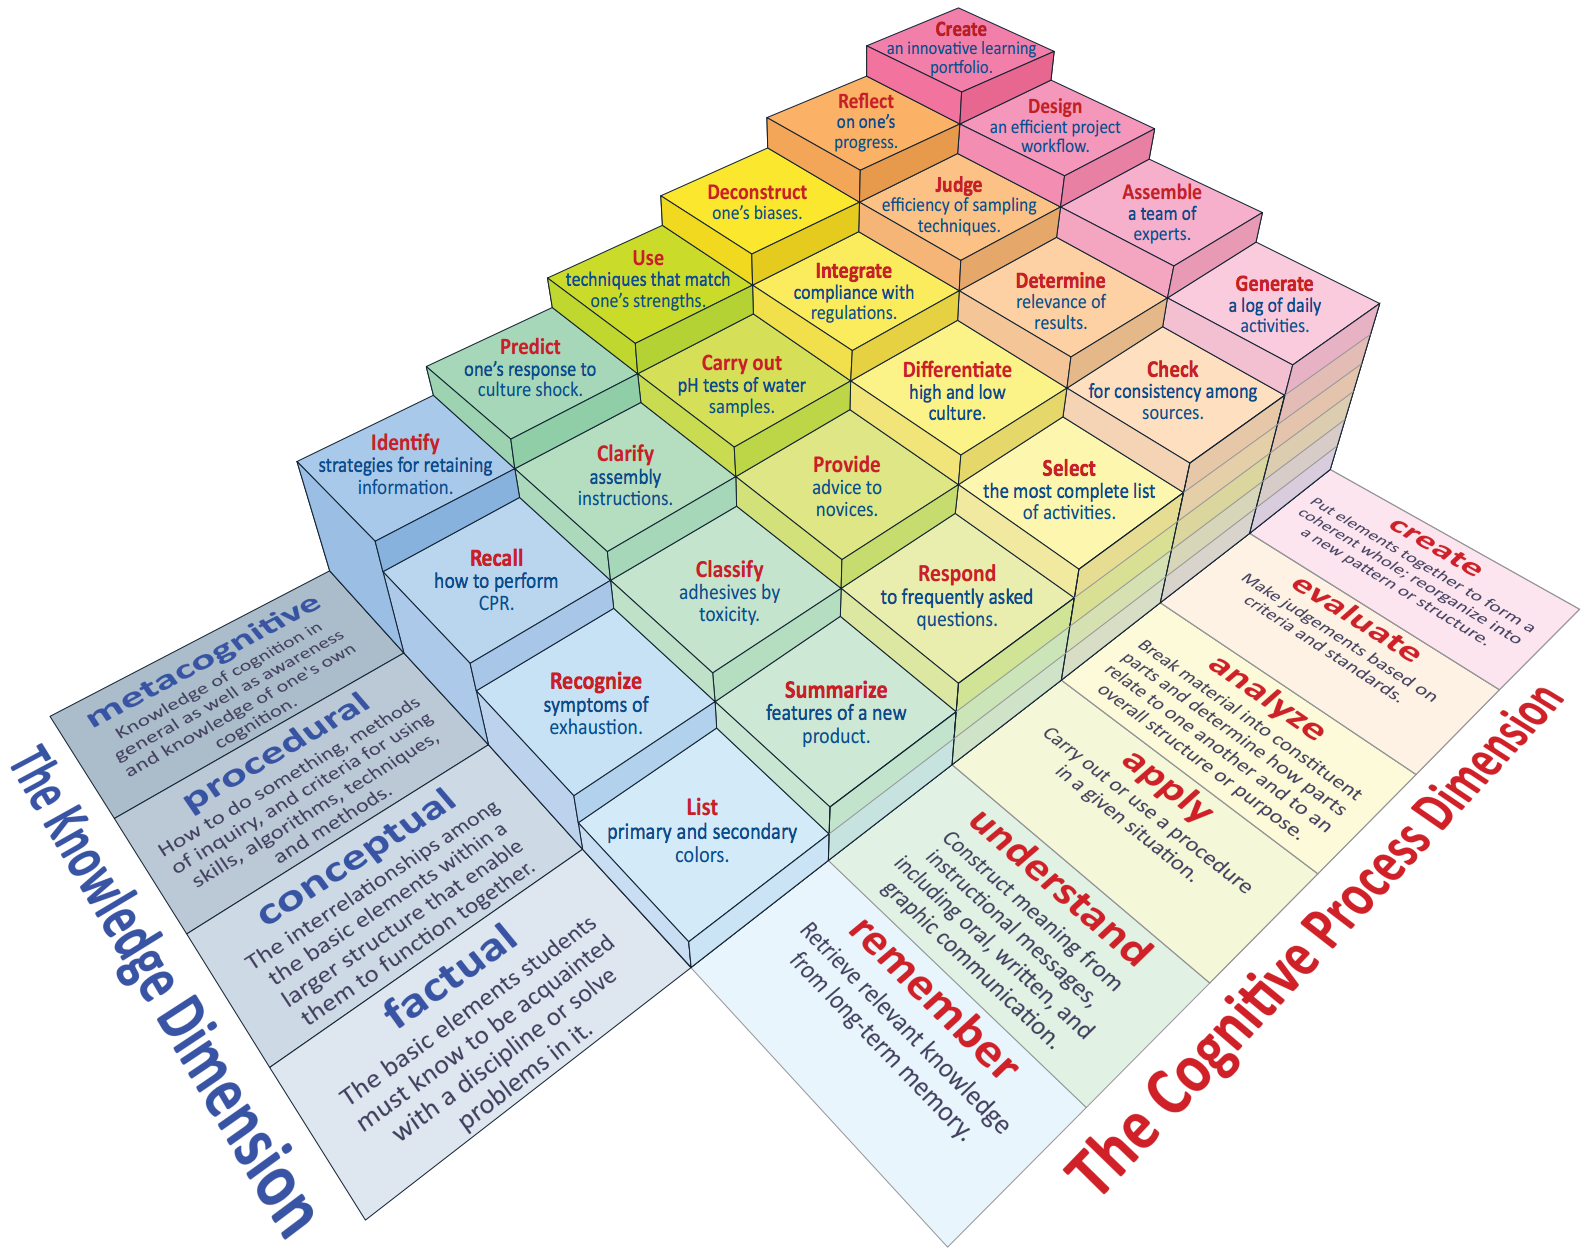
\includegraphics[width=1.0\textwidth]{RevisedBloom.png}
    \caption{Bloom's revised taxonomy visualised with examples of different learning objectives.}
    \label{fig:revised-bloom}
\end{figure}

  Learning activities often involve both lower order and higher order thinking skills as well as a mix of concrete and abstract knowledge.

  The taxonomy can provide usable insight into how to design, by the combination between lower or higher cognitive complexity, and concrete (factual or conceptual) or abstract knowledge (procedural or metacognitive). \cite{cheong}

  \subsubsection{Building skills: by Spaced practice, Deliberate practice and Perceptual exposure}

  Spaced practice deals with spreading out learning, with the purpose of not forgetting. E.g. Gates \cite{Gates} concludes that spaced learning versus massed learning did have a memory benefit in their study.

  Designing for this, could mean making the user apparent on the person's meta-cognitive ability (personal insight into what you'll remember), and meta-memory (when you need to repeat information in order not to forget).

  Moreover, dividing learning into 45-90-minute chunks, getting to 95\% reliable within three sessions, has been proven highly effective. This is called deliberate practice. Gates \cite{Gates} agrees, finding no evidence of consistent correlation between total duration and effects on learning outcomes in their study.

  Sierra presents a number of strategies, most notably research within deliberate practice \cite{yengin} \cite{sierra}. Deliberate practice has been proven to be an effective way to build skills. It has also been tested before for mobile learning environments. \cite{yengin}

  Sierra \cite{sierra} suggests skills to be divided into three buckets: can't do (but need to do), can do with effort, and mastered (reliable/automatic). The goal then is to move skills from can't do into mastered, in the best way possible. See figure \ref{fig:sierra-practice} from Sierra \cite{sierra}.

  \begin{figure}[h]
    \centering
    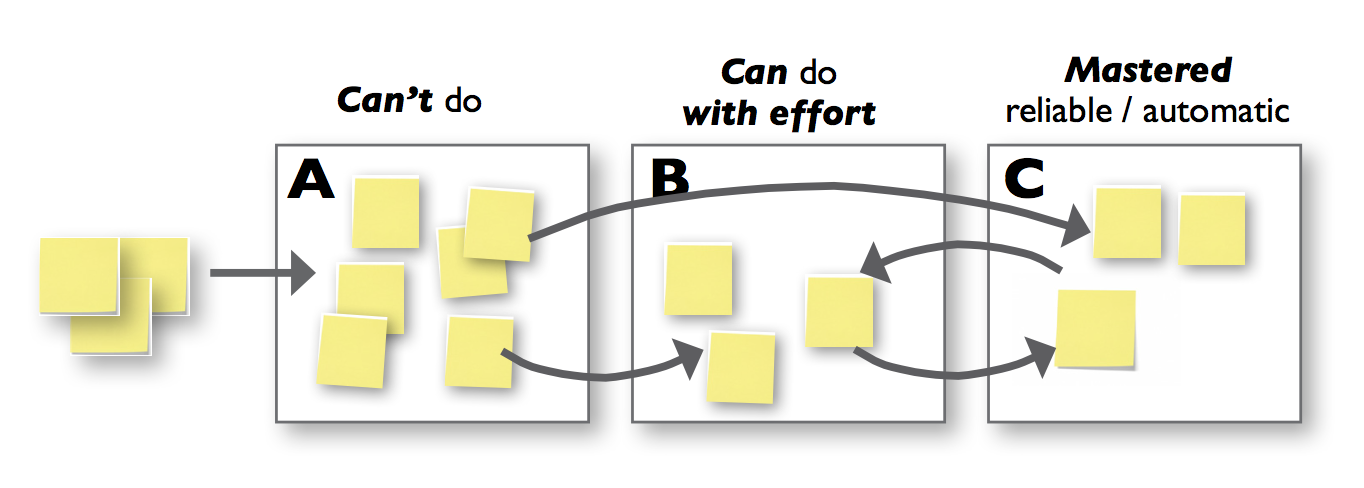
\includegraphics[width=0.8\textwidth]{SierraPractice.png}
    \caption{Moving skills from A (Can't do) to B (Can do with effort) into C (Mastered) can move different ways, depending on how effective the learning is. Deliberate practices focuses on A-B-C, while perceptual expose enables A to C. Reflection allows knowledge to go backwards, to get better at the skill than previously possible.}
    \label{fig:iterationprocess}
\end{figure}

  Desirable difficulties applies here, meaning that during deliberate practice, it may feel as if learning gets harder and harder, but in the long term the user is actually learning more. As a result, less people does true deliberate practice, but they do not get the same reward in return. This needs to be designed for, e.g. using social psychology.

  A way to build skills quickly, is to utilize that the brain is brilliant at pattern-matching, by the method "perceptual exposure". \cite{sierra}

  By exposing users to very high-quality samples during a very limited time, experts can learn intuitively.

  \subsubsection{Learning from Assessment}

  Knowing what learners know, and don't know, is crucial to effective learning, Luckin \cite{luckin} says.

  Assessment can partly help to design for flow, matching challenge and ability \cite{bruhlmann}, which is effective for intrinsic motivation (see next chapter).

  Moreover, it also has cognitive benefits. It can help to offer appropiate feedback, increase learners' awareness of their learning needs, and give accurate assessment and analysis, and allows learning to be tailored.

  By recognizing differences of students, in their ability to understand what they know and how they can progress, it is possible to ensure that everyone achieves their full potential.

  Effective assessment by a teacher or agent includes individual feedback (task-oriented and informal) and appropiate feed-forward advice.

  \subsubsection{Learning by Thinking: Reflection \& Retrieval Practice}

  When reflecting, the student develops neccessary skills and self-awareness to refine their own learning activities. This surely applies to the teacher as well, Luckin says. \cite{luckin}

  Stefano \cite{stefano} suggests that that reflection has been an overlooked area of research for a long time.

  They found that individuals who are given time to reflect on a task, outperforms students who are given the same amount of time to practice with the same task.

  His results suggests that reflection as an activity that can be more effective than additional learning.

  Similar to deliberate practice, it is a desirable difficulty. Individuals in the test themselves, had a tendancy to allocate time to practice on the task rather than reflecting on it.

  %\subsubsection{Retrieval practice}

  Bjork \cite{bjork} shows that retrieval from memory is more effective than people who repeat reading the same thing to remember.

  They also showed, that the more effective students, retrieves from memory.

  E.g. "What was in that article?", instead of immediately reading the article, is an example of memory retrieval that is extremely effective for learning, their research shows.

  One design method to encourage this, would be flip cards, where the question is on one side, the answer is on the other, versus giving the person a multiple-choice question.

%\subsubsection{Not forgetting}

%UCLA Bjork's Learning and Forgetting Lab researches how people forget, and how to design so that people do not forget.

%\include{theory/learning/pedagogical-development/social_psychology}

